\vspace*{4cm}
\part{Zigbee}\label{part:Zigbee}
Autor: Cyrill Horath
\vspace*{\fill}
\clearpage

\section{Einleitung}\label{sec:EinleitungZigbee}
In diesem Teil der Arbeit werden die Eigenschaften und Besonderheiten des Zigbee Mesh Stack erläutert und es wird auf die Umsetzung des Benchmarks auf Stack Ebene eingegangen. Dieser Teil soll als eigenständiger Teil betrachtet werden in dem ausschliesslich Zigbee behandelt wird.

\begin{wrapfigure}{r}{0.5\textwidth}
	\centering
	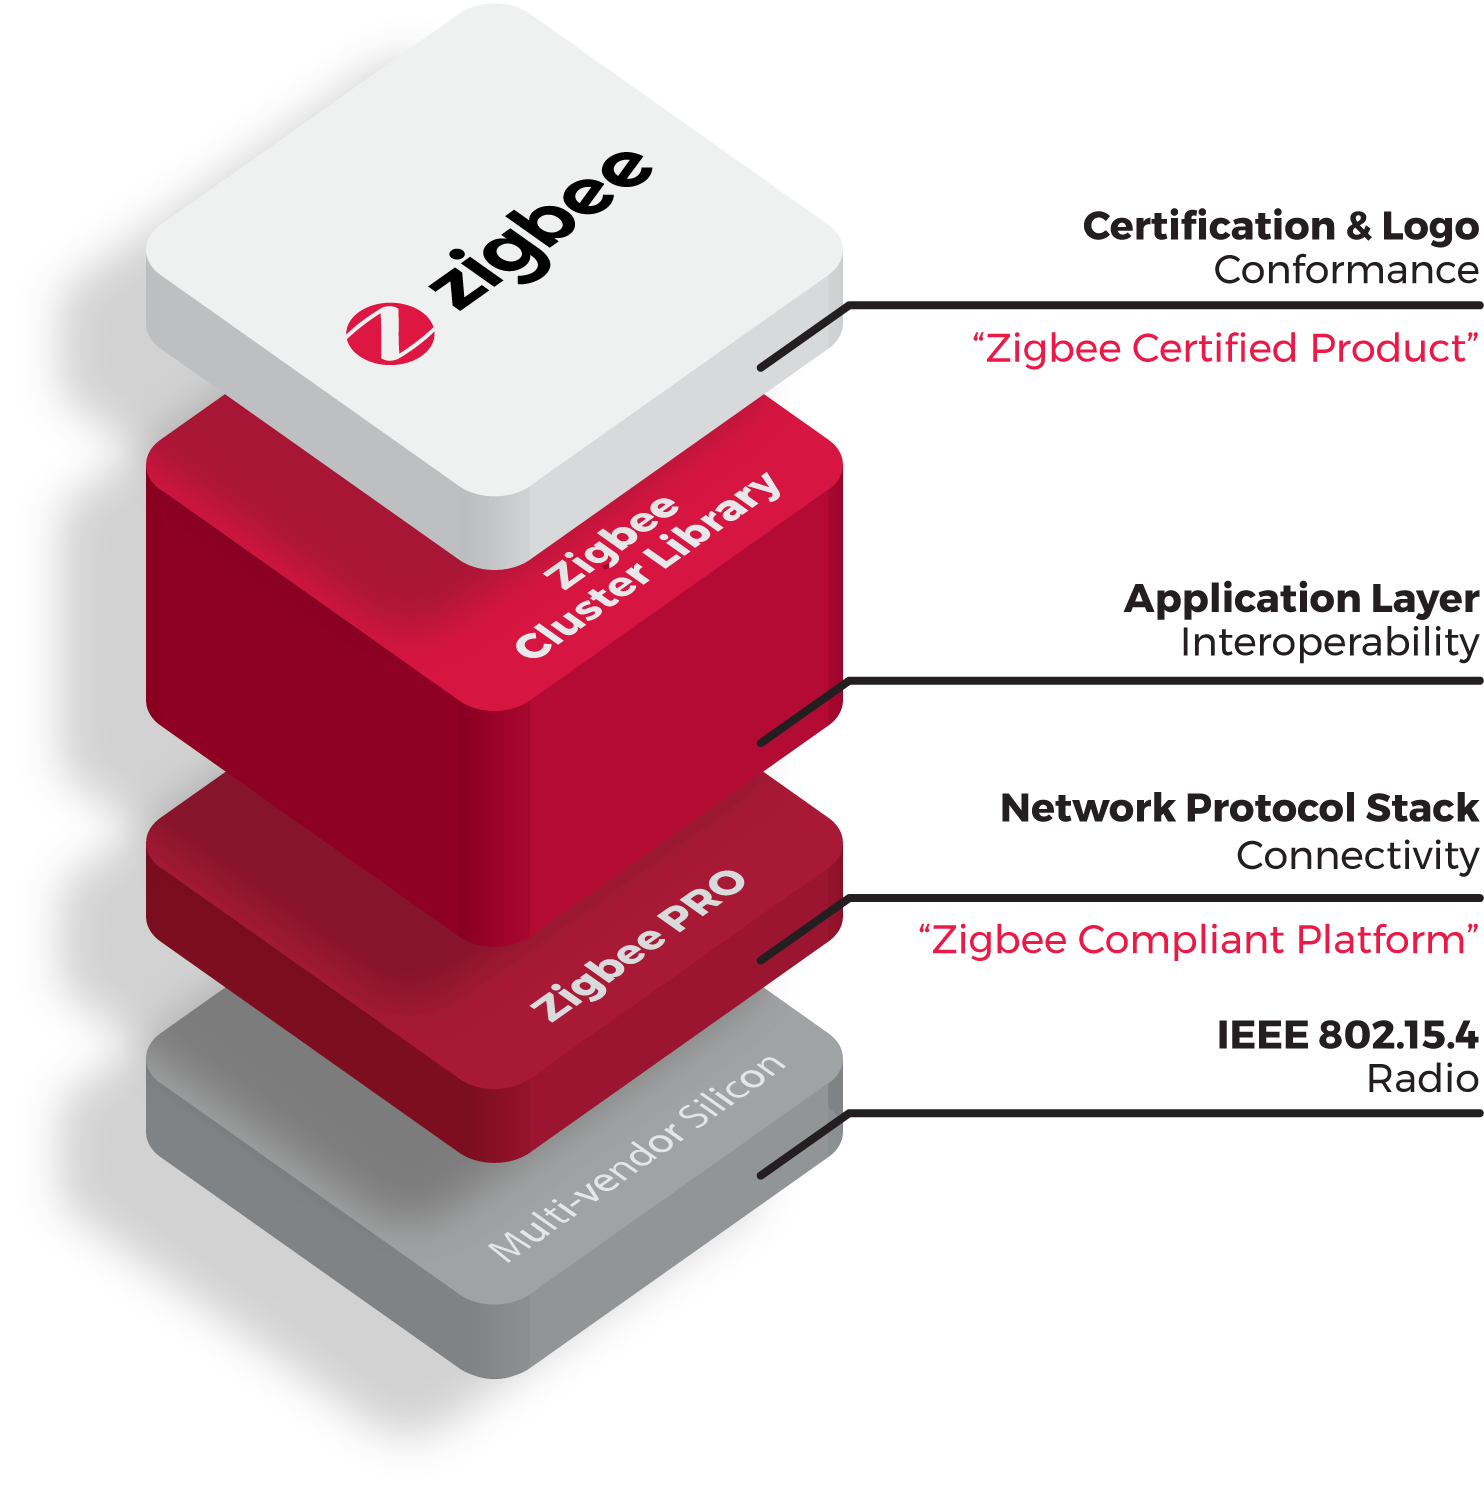
\includegraphics[width=0.5\textwidth]{Zigbee_Stack_symbolic.png}
	\caption{Zigbee Protokollstack}	\label{fig:ZigbeeProtokollstack}
\end{wrapfigure}

Zigbee ist ein auf dem IEEE 802.15.4 Standard aufbauendes drahtloses Low Power Mesh Netzwerk. Es nutzt das vom IEEE 802.15.4 Standard definierte ISM-Funkfrequenzband 2.4GHz plus weitere Sub-GHz Bänder je nach Region.
Die im Jahre 2002 gegründete Zigbee Allianz spezifiziert den Protokoll Standard und gibt seit da an laufend Neuerungen und Updates heraus.
Im Zuge der Verbreitung von Technologien in der Heim Automatisierung erhielt auch Zigbee immer mehr Aufmerksamkeit und wuchs bis heute zum wohl am weitesten verbreiteten Mesh Netzwerk Protokoll in diesen Gebiet heran. Besonders in Systemen für die Steuerung von Beleuchtungen wie zum Beispiel Phillips Hue und Ikea Tradfri kommt Zigbee verbreitet zum Einsatz.

Die Spezifikationen innerhalb des Zigbee Protokollstacks sind weitreichend. Von der MAC Ebene über die Netzwerkschicht bis hin zur Applikationsebene gibt es klare Vorgaben wie ein Zigbee Produkt aufgebaut sein soll.
Mit der \textit{Zigbee Cluster Library} werden sogar spezifische Anwendungen vordefiniert wie beispielsweise die Steuerung eine Lichtquelle mit Dimmfunktion.
Diese Spezifikationen ermöglichen die Interoperabilität von Systemen mit der gleichen Funktion jedoch von unterschiedlichen Herstellern.



%\begin{figure}[h]
%	\centering
%	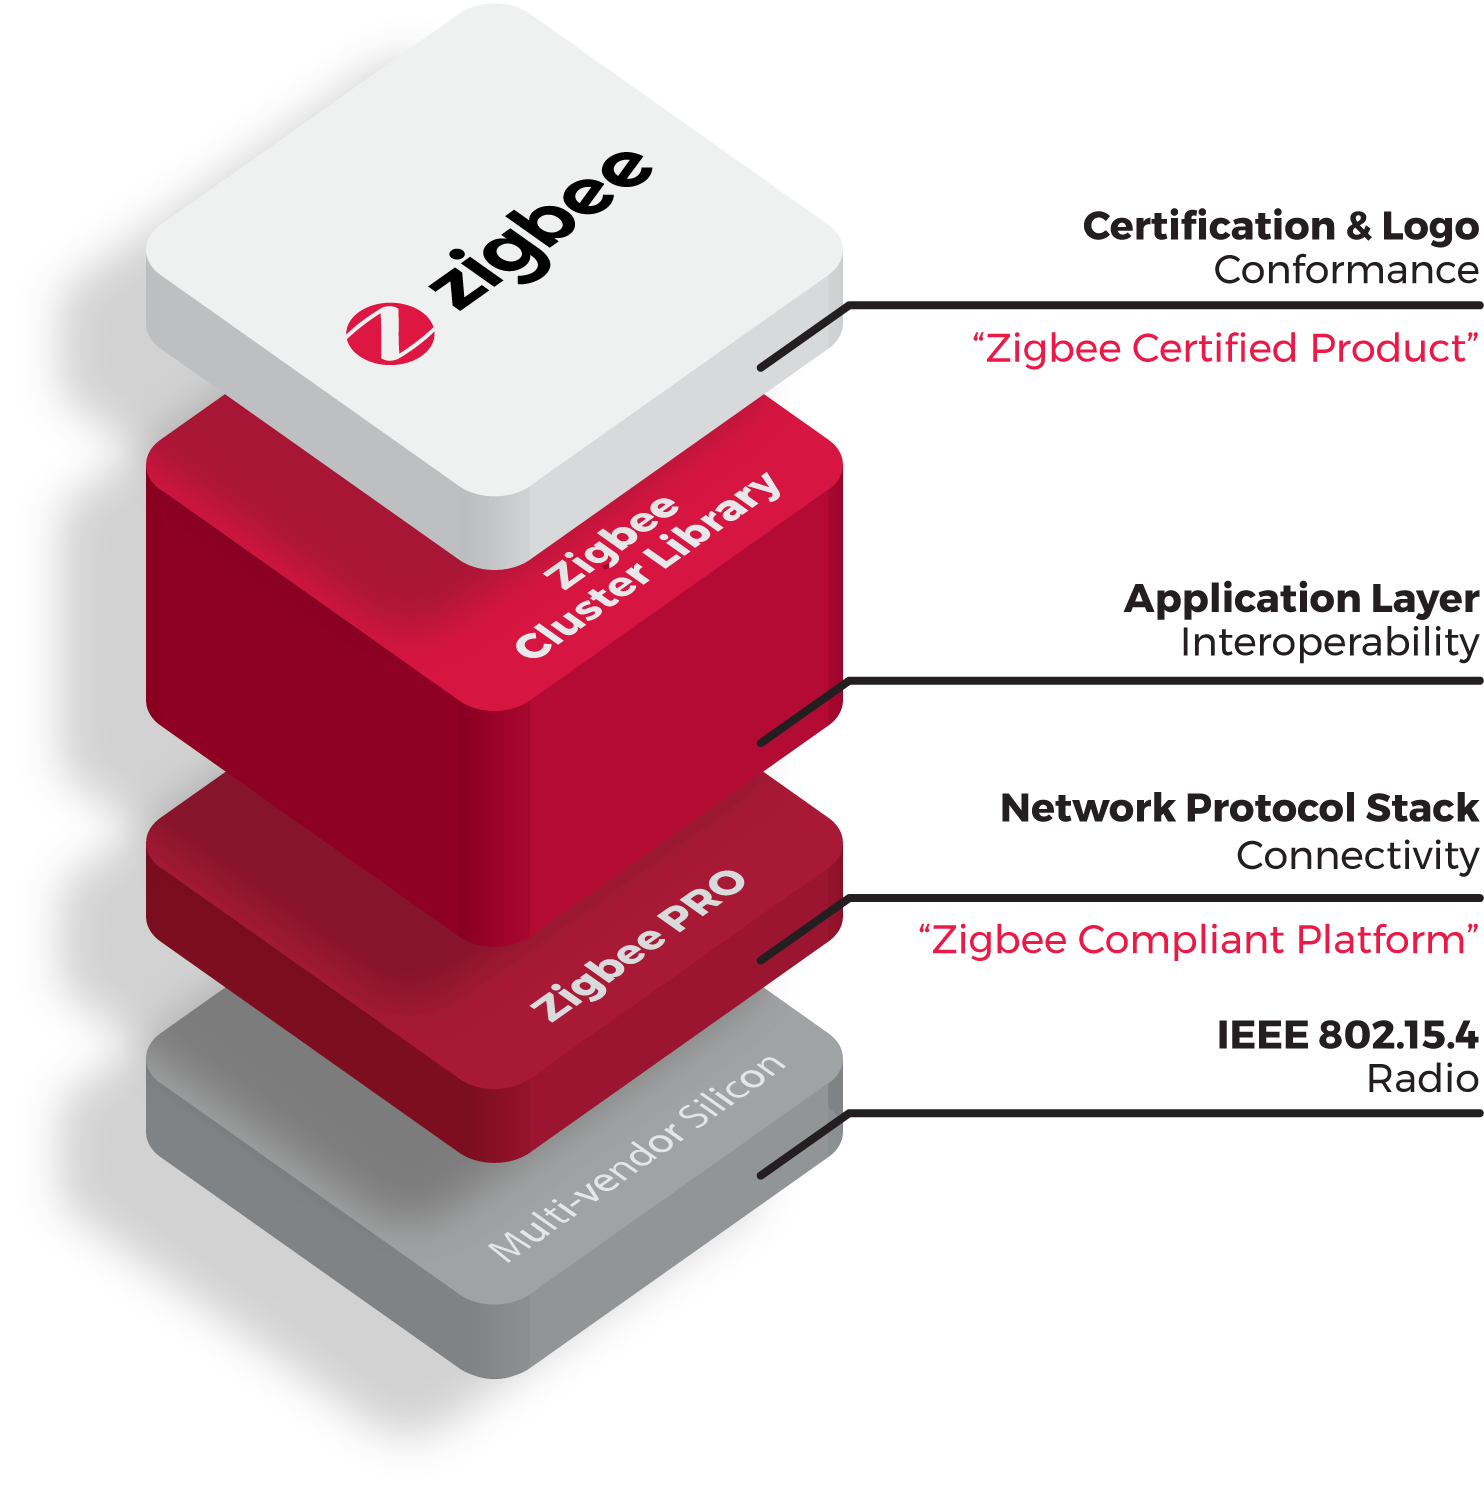
\includegraphics[width=0.8\textwidth]{Zigbee_Stack_symbolic.png}
%	\caption{Zigbee Protokollstack}	\label{fig:ZigbeeProtokollstack}
%\end{figure}



